\documentclass[12pt, a4paper]{article}
\usepackage{scrextend}
\usepackage{titlesec}
\usepackage{graphicx}
\usepackage{amsmath}
\usepackage{amsfonts} % for the real number symbol
\usepackage{geometry}
\usepackage[unicode]{hyperref}
\usepackage{titlesec}
\usepackage{titletoc}
\usepackage[sorting=none]{biblatex}
\usepackage{enumitem}
\usepackage{indentfirst}
\numberwithin{equation}{section} % number equations by section
\renewcommand{\figurename}{Att.}
\renewcommand{\contentsname}{Saturs}
\renewcommand{\labelenumi}{\arabic{enumi})} % lists with 1)
\setlist{nosep}
\parindent=1cm
\linespread{1.213} % equivalent to 1.5 in word, experimentally.
\addbibresource{refs.bib}

\geometry{
    a4paper,
    lmargin=30mm,
    rmargin=20mm,
    tmargin=20mm,
    bmargin=20mm
}


\titleformat{\section}
    {\normalfont\large\bfseries}{\thesection . }{0.2em}{\MakeUppercase}
\titleformat{\subsection}
    {\normalfont\large\bfseries}{\thesubsection . }{0.2em}{}
\titleformat{\subsubsection}
    {\normalfont\normalsize\bfseries\itshape}{\thesubsubsection . }{0.2em}{}
\titlespacing*{\subsubsection}{0pt}{6pt}{0pt}

\begin{document}
\begin{titlepage}
    \begin{center}
        \vspace*{3cm}
        
        LATVIJAS UNIVERSITĀTE

        DATORIKAS FAKULTĀTE

        \vspace*{4cm}

        \large\textbf{ATDARINOŠĀS MAŠĪNMĀCĪŠANĀS PIELIETOJUMS ROBOTIKĀ}
        
        \vspace{2cm}
        \normalsize{MAĢISTRA KURSA DARBS}
         
             
    \end{center}
    \vspace{3cm}
    \begin{addmargin}[18em]{0em}
    Autors: \textbf{Pēteris Račinskis}
    \end{addmargin}

    \begin{addmargin}[18em]{0em}
    \hspace{1cm} Stud. apl. Nr. pr20015
    \end{addmargin}

    \begin{addmargin}[18em]{0em}
    Darba vadītājs: Dr. sc. comp. Modris Greitāns
    \end{addmargin}
         
    \vfill
    \begin{center}
    RĪGA 2022
    \end{center}
 \end{titlepage}
\newpage
\tableofcontents
\thispagestyle{empty}
\newpage
\setcounter{page}{3}


\section{Ievads}

Sacīt, ka mašīnmācīšanās šobrīd ir ļoti aktuāla pētniecības nozare, būtu maigi. Pēdējās desmitgades laikā tieši šis izpētes lauks ir eksplodējis popularitātē kā neviens cits, pateicoties galvenokārt diviem faktoriem: ļoti vispārīgiem neironu tīklu modeļiem un skaitļošanas resursu veiktspējai, kas beidzot ļāvusi šos teorētiski jau ļoti sen\cite{mcculloch1943logical, linnainmaa1970representation, fukushima1988neocognitron} iedomātos mākslīgā intelekta uzbūves elementus realizēt praksē. Tā risināti uzdevumi, ko izsenis daudzi uzskatījuši par neiespējamiem, un lietojuši kā argumentu pret mašīnmācī-šanos kā rīku, kas spētu konkurēt ar bioloģiskas izcelsmes prātiem --- semantiskas nozīmes meklēšana attēlos\cite{krizhevsky2012imagenet}, tekstu korpusu analīze un ģenerēšana ar "izpratni" par to satu-ru\cite{vaswani2017attention} un visspējīgāko spēlētāju pārspēšana nepilnīgas informācijas spēlēs ar neaptverami milzīgiem iespējamo stāvokļu permutāciju skaitem\cite{silver2016mastering}.

Nav arī īpaši grūti atrast vēsturisko saikni starp mākslīgo intelektu un robotiku. Tautas iztēlē termins ``robots'' drīzāk droši vien iezīmēs zinātniskās fantastikas radītos personāžus --- mehāniskas būtnes, kas spēj patstāvīgi darboties neierobežotā vidē un risināt sarežģītus uzdevumus --- nevis pieticīgākus, reāli pastāvošus un ražotnēs rodamus industriālos robotus. Un šī pati zinātniskā fantastika radījusi arī nesaraujamu saiti starp robotiem un mākslīgo intelektu\cite{asimov2004robot} --- diskusijas par mākslīgo intelektu bieži plūstoši pāriet diskusijās par ar šādu intelektu aprīkotiem robotiem, un šo robotu neizbēgami kareivīgajām ambīcijām attiecībā pret cilvēci. Protams, zinātne ne vienmēr seko populār-zinātniskās iedomas lidojumam, taču šāda saikne ir visnotaļ pamatota --- spēja mācīties no paraugiem vai patstāvīgi un pielāgoties savai apkārtnei ir ārkārtīgi noderīga, jo daudzi uzdevumi, kuru risināšanai varētu pielietot robotus, ir sarežģīti nevis to fizikālajā izpildē, bet tieši vadības uzdevuma formulēšanā un realizācijā.

Atdarinošā mašīnmācīšanās (\textit{imitation learning}) ir viens no paņēmieniem, ar kuriem tiek mēģināts risināt šādas sarežģītas vadības problēmas. Lai gan pamatu pamatos nevar apgalvot, ka tā ir tikai robotikai piemērota metožu saime, lielākā daļa izpētes virzīta tieši šajā virzienā --- problēmas tiek formulētas kā fizikālu (vai nosacīti fizikālu --- virtuālās vidēs simulētu) procesu kontroles uzdevumi, un risinājumi tiek rasti no pēc iespējas mazāka skaita veiksmīgas darbības piemēru. Mašīnmācīšanās nozarē bioloģiskas analoģijas un iedvesma nav nekāds retums, un savā ziņā šāda mācīšanās  atspoguļo vienu no izplatītiem paņēmieniem, kā cilvēki vai sabiedriski dzīvnieki nodod prasmes viens otram - demonstrējot. Nevar nepieminēt, ka izpēte šajā jomā bieži aizņemas pieejas un iespaidojas no rezultātiem, kas gūti ar stimulēto mašīnmācīšanos (\textit{reinforcement learning}) - savā ziņā vispārīgu, pašmācībai un treniņam analoģisku paņēmienu. Arī abu metožu apvienojums ir ideja, kas pavīd visai regulāri --- cerībā, ka, atdarinot ekspertus, var ātrāk nonākt pie derīgām stratēģijām, kas var kalpot kā sākumpunkts dziļākai pašmācībai; vai arī izmantot šādu stimulēto metodi, lai precīzāk imitētu treniņa datus.


\subsection{Darba mērķis un struktūra}

Šis ir maģistra kursa darbs - pirmais konkrētais rezultāts, kas sasniegts maģistra darba izstrādes procesā. Tāpēc ir jārēķinās ar diezgan īpatnēju formātu un saturu - tiek dokumentēta kāda pētnieciska projekta pirmā fāze, kas bieži vien sastāv no dažādu literatūras avotu izpētes un personiskiem treniņiem, vēl pirms iespējams nopietni sākt eksperimentālu darbību vai pat izvirzīts konkrēts mērķis visam projektam.

Arī šis gadījums nav nekāds izņēmums. Sākumā izvēlēta ļoti aptuvena tēma, balstoties uz Elektronikas un datorzinātņu institūta ekspertu ieteikumiem, un pirmajā darba semestrī lielākoties veikta attiecīgās nozares apguve pašmācības ceļā. Šī nodarbe sastāvē-jusi galvenokārt no divu veidu darbībām --- zinātniskās literatūras lasīšanas un tajā aprakstīto teorētisko jēdzienu un praktisko metožu apguves ar vienkāršiem eksperimentiem personiskās izpratnes veicināšanai.

Līdz ar to šīs atskaites galvenais mērķis ir sniegt ieskatu līdz šim maģistra darba gatavošans ietvaros paveiktajā un apgūtajā. Tā sastāv no trim galvenajām daļām:
\begin{enumerate}
    \item ievada, kurā īsi izklāstīti vispārīgi jēdzieni, kas nepieciešami, lai izprastu zinātnisko literatūru nozarē;
    \item pētniecisku rakstu izlases iztirzājuma un salīdzinājuma;
    \item neliela apraksta par paša veikto darbību, apgūstot mašīnmācīšanās modeļus un to realizācijai nepieciešamo programnodrošinājumu.
\end{enumerate}


\subsection{Terminoloģijas tulkojumi}

Viena no īpatnībām, ar ko ir nācies saskarties, strādājot tieši ar mašīnmācīšanās nozari, ir nepārprotamas terminoloģijas trūkums latviešu valodā. Pati zinātnes nozare, lai arī nebūt ne tik jauna kopumā, piedzīvojusi milzīgas izmaiņas un nepieredzētu uzplaukumu pēdējās desmitgades laikā. Protams, datorzinātnes laukā pirmā un galvenā saziņas valoda ir angļu. Attiecīgi novērajami divējādi un saistīti fenomeni - publikācijas un terminoloģija, kas radītas senāk, veidojušas dziļi specifisku nišu, kas nav iedvesmojusi daudz mēģinājumu tulkot to uz citām valodām, savukārt uzplaukuma laikos vēl ir ļoti daudz materiāla, ko vienkārši neviens nav paguvis iztulkot.

Patvaļīgi izvēloties tulkojumu, pastāv risks mulsināt lasītāju un sadrumstalot jau tā nelielo literatūras kopu dažādu atslēgas vārdu izvēles rezultātā. Tāpēc šeit izveidots saraksts ar potenciāli mulsinoši tulkoto terminoloģiju tās oriģinālajā formulējumā angļu valodā, izvēlētajiem tulkojumiem un īsiem pamatojumiem.  

\begin{enumerate}
    \item \textit{policy} --- \textbf{stratēģija}. Šis termins pamatā tiek lietots, lai aprasktītu kādu funkciju, kas novērojumus attēlo lēmumu telpā. Pirmais ieraksts tieši tāpēc, ka varētu būt strīdīgākais. Angļu valodā pastāv divi termini, \textit{policy} un \textit{politics}, kas parasti latviski tiek tulkoti vienādi --- politika --- par spīti radikāli atšķirīgām nozīmēm. Termins \textit{strategy} tiek lietots kā sinonīms pirmajam abās valodās, un arī piemērojams tieši šādām lēmumu pieņemšanas funkcijām, piemēram, spēļu teorijā.
    \item \textit{reinforcement learning} --- \textbf{stimulētā mašīnmācīšanās}. Meklējumi tiešsaistē atklāj \cite{enc_stim}, ka šis tulkojums jau ir samērā izplatīts, taču varētu būt nezināms lasītājiem, kas ar to sastopas pirmo reizi --- pat ja zināms metodes angliskais nosaukums.
    \item \textit{imitation learning} --- \textbf{atdarinošā mašīnmācīšanās}. Paša autora piedāvāts tulkojums, izmantojot iepriekšējo kā piemēru, jo nav izdevies atrast alternatīvas. Latvis-kais vārds "atdarināt" izvēlēts pār internacionālismu ``imitēt'', jo to vieglāk izlocīt formā, kas neizklausās lauzīta un neveikla. Taču procesā zūd spēja viegli atrast sākotnējo vārdu svešvalodā, kas ļoti svarīga zinātniskajā vidē, kurā latviski pie-ejamo resursu ir maz.
\end{enumerate}

\subsection{Tehniskās priekšzināšanas, definīcijas}

Pētot un veidojot spriedumus par zinātnisko literatūru viens no lielākajiem šķēršļiem lasītājam ``no malas'' ir katrā nozarē pieņemtais tehnisko priekšzināšanu kopums, ko autori sagaida no auditorijas. Tas, protams, ir loģiski, jo publikācija, kas apraksta jaunākos atklājumus kādā dziļi specifiskā lauciņā, nevar veltīt visu sev atvēlēto drukas apjomu elementāras un vispārzināmas terminoloģijas skaidrojumiem. Tāpat, tālāk atskaitē iztirzājot šos rakstus, noderīgi ir ieviest tiem kopīgus apzīmējumus un definēt visus vienuviet.

\subsubsection{Parametriski modeļi, šabloni}

Viens no visplašāk izmantotajiem formālismiem datizraces un mašīnmācīšanās lau-kos ir parametriskais modelis. Pamatā tam ir ideja, ka nezināmu funkciju, kuras rezultātus vēlamies paredzēt, var aproksimēt ar citu funkciju jeb modeli:

\begin{equation} 
    M(x) \approx f(x)
\end{equation}

Protams, šādu modeļu varētu būt bezgalīgi daudz, un tie visi var atšķirties pēc tā, cik labi spēj paredzēt nezināmās funkcijas vērtības. Tāpēc modeļu meklēšanai parasti izmanto šablonus - funkcijas, kuru argumentā papildus ievades datiem ir brīvi maināmi un kopīgi (tātad "apmācāmi") parametri $\theta$:

\begin{equation} 
    \text{Meklē } \theta:M(x \vert \theta) = M_{\theta}(x)  \approx f(x)
\end{equation}

Iegūtā šablona funkcijas un apmācīto parametru kombinācija $\lbrace M, \theta \rbrace$ tad veido konk-rētu modeli. Labs šablons ir tāds, kas spēj pielāgoties ļoti daudzām dažādām funkcijām:

\begin{equation} 
    \forall f \forall x \exists \theta:M_{\theta}(x)\approx f(x)
\end{equation}

Atkarībā no uzdevuma specifikas, izplatīti modeļi mēdz būt regresori, kas aproksimē (parasti vektoriālas) funkcijas ar skaitliskām vērtībām,

\begin{equation} 
    f:x \rightarrow \mathbb{R}^k
\end{equation}
\begin{equation} 
    M: x \times \theta \rightarrow \mathbb{R}^k
\end{equation}

un klasifikatori, kas paredz ievades datu punkta piederību kādai diskrētai klasei

\begin{equation} 
    f:x \rightarrow C = \lbrace c_1, c_2, ..., c_m \rbrace
\end{equation}
\begin{equation} 
     M: x \times \theta \rightarrow C
\end{equation}

Bieži vien noderīgi ir ne tikai spēt attēlot datu punktu kā diskrētu klasi, bet iegūt varbūtību sadalījumu, kas apraksta tā iespējamību piederēt jebkurai no klasēm:

\begin{equation} 
    M: x \times \theta \times c_i \rightarrow [0; 1]
\end{equation}
\begin{equation} 
    M_{\theta}(x, c_i) = P_i
\end{equation}
\begin{equation} 
    \sum_{i=1}^m P_i = 1
\end{equation}

Lai varētu novērtēt, cik labi modelis aproksimē nezināmo funkciju, un vadīt parame-tru apmācības procesu, tiek izmantotas mērķa funkcijas (\textit{loss functions})\cite{notation}:

\begin{equation} 
    \ell: M_{\theta}(x) \times f(x) \rightarrow \mathbb{R}
\end{equation}

Strādājot ar reāliem datiem, datu punkti veido datu kopu, kas parasti tiek uzskatīta par gadījuma izlasi no punktus ģenerējošā varbūtību sadalījuma. Praktiskiem apmācības uzdevumiem datu kopa parasti jāiegūst formā, kas satur gan sagaidāmos ievades datus, gan pareizu rezultātu:

\begin{equation} 
    s \sim \mathcal{D} \Leftrightarrow s \text{ ir no varbūtību sadalījuma } \mathcal{D}
\end{equation}
\begin{equation} 
    y_i = f(x_i)
\end{equation}
\begin{equation} 
    s_i = (x_i, y_i)
\end{equation}
\begin{equation} 
    S = \lbrace s_1, s_2, ..., s_n \vert s_i \sim \mathcal{D}\rbrace
\end{equation}

Datu kopai var aprēķināt empīrisku mērķa funkcijas novērtējumu,

\begin{equation} 
    L_S(\theta) = \frac{1}{n}\sum_{i=1}^n\ell(M_{\theta}(x_i), y_i)
\end{equation}

bet apmācības process parasti kādā veidā tiecas minimizēt šīs vērtības matemātisko cerību ģenerējošam sadalījumam (nevis tikai pašai datu kopai - ja modelis ļoti cieši pielāgots konkrētai datu izlasei bet zaudē precizitāti sadalījumam kopumā, to sauc par pārpielāgošanos --- \textit{overfitting})

\begin{equation} 
    L_{\mathcal{D}}(\theta) = \mathbb{E}_{\mathcal{D}} [\ell(M_{\theta}(x_i), y_i)]
\end{equation}
\begin{equation} 
    \text{Apmāca } M_{\theta} \text{ uz } \mathcal{D} \rightarrow \text{Minimizē } L_{\mathcal{D}}(\theta)
\end{equation}

Ja modelis ir stratēģija (\textit{policy}), stimulētās vai atdarinošās mašīnmācīšanās literatūrā to ļoti bieži izsaka kā $\pi_{\theta}(x)$. Mazliet mulsinošs ir tieši ar imitējošām metodēm saistītos rakstos lietotais apzīmējums $\pi^*$, ar ko apzīmē t.s. ``ekspertu stratēģijas'' --- kas pašas ir nezināmās funkcijas, ko cenšamies aproksimēt pēc to ģenerēto punktu kopām. 


\subsubsection{Neironu tīkli}

Neironu tīkls ir izplatīta modeļu šablonu saime, ko var izmantot dažādas formas funkciju aproksimēšanai --- tie var būt gan klasifikatori, gan regresori, un pastāv ļoti dažādas to uzbūves variācijas, kas daļēji teorētiski, daļēji empīriskas eksperimentācijas rezultātā un daļēji kopējot bioloģiskās sistēmās atrodamas struktūras izstrādātas dažādu uzdevumu veikšanai. Neironu tīklu kopīgais elements ir t.s. perceptorns, kas izteikts jau pašos pirmsākumos\cite{mcculloch1943logical}. Perceptrons funkcija, kas piemēro nelineāru aktviācijas funkciju $\sigma$ argumentu vektora $\vec{x}$ elementu savstarpējai lineārai kombinācijai, t.i,


\begin{equation} 
    f_{perceptron}(\vec{x}) = \sigma(\vec{w} \cdot \vec{x}+b)
\end{equation}

kur $\vec{w}$ ir t.s. svaru vektors, bet $b$ ---  nobīde. Perceptrona parametri tātad ir brīvie mainīgie $\vec{w}$ un $b$. Neironu tīkls parasti sastāv no slāņiem --- perceptronu $f_i$ kopām, kas visi apstrādā to pašu argumentu vektoru, bet katrs ar saviem parametriem $\vec{w}_i,b_i$. Tad slāni algebriski izsaka formā

\begin{equation} 
    W = \begin{bmatrix}
        w_1^T \\
        w_2^T \\
        ... \\
        w_k^T
    \end{bmatrix}; 
    \vec{b} =  \begin{bmatrix}
        b_1 \\
        b_2 \\
        ... \\
        b_k
    \end{bmatrix}; 
\end{equation}
\begin{equation} 
    f_{layer}(\vec{x}) = \sigma(W\vec{x}+\vec{b})
\end{equation}

Ja slānis tīklā ir pēdējais un tā vērtības ir modeļa izvadē, to sauc par izvades (\textit{output}) slāni. Ievades datu vektoru sauc par ievades (\textit{input}) slāni. Pārējos slāņus sauc par slēptajiem (\textit{hidden layers}). Saka, ka slāņi savā starpā pilnīgi savienoti (\textit{fully connected}), ja katram viena slāņa perceptronam argumentā parādās visi iepriekšējā slāņa izvades elementi. Svarīga neironu tīkla īpašība --- ja tā aktivācijas funkcijas ir diferencējamas, tad arī tīkls kopumā ir diferencējams pēc katra tā parametra, pat ar perceptroniem daudzos slāņos. Līdz ar to var izmantot t.s. \textit{backpropagation} algoritmu, kas atrod mērķa funkcijas parciālos atvasinājumus pēc modeļa parametriem un izmanto kādu gradientu optimizācijas metodi apmācībai.

Pastāv dažādas šo tīklu arhitektūras. Vienkāršākās sastāv no viena vai vairākiem slāņiem (neskaitot ievades slāni), taču ir plaši izplatīti arī, piemēram, konvolucionālie neironu tīkli\cite{krizhevsky2012imagenet}, ko izmanto attēlu apstrādē, tai skaitā šajā atskaitē aplūkotajos pētījumos, kur nepieciešams gūt informāciju no video datiem. Galvenā atšķirība konvolucionālajā tīklā ir t.s. kodola funkciju jeb kerneļu (\textit{kernel}) izmantošana - konvolucionāli slāņi vienā līmenī piemēro identiskas perceptrona funkcijas nelieliem iepriekšējā slāņa (matricas vai tenzora formā) reģioniem. Tas palīdz identificēt dažādas lokālas struktūras, piemēram, attēlā. Šo un vēl citu veidu sarežģītāku neironu tīklu arhitektūra ir ļoti plašs lauks, ko detalizēti šeit iztirzāt nav iespējams.

\subsubsection{Markova lēmumu procesi}

Pastāv dažādi formālismi procesu definēšanai vadības sistēmu izstrādes mērķiem, lai ar tiem varētu veikt matemātiskas operācijas. Izplatīti atdarinošās un stimulētās mašīnmācīšanās literatūrā ir Markova lēmumu procesi (MDP --- \textit{Markov decision processes}), kas izmantojami situācijās, kad sistēmas stāvokli nākotnē pilnībā nosaka pašreizē-jais. Dažādi autori, kas darbojas dažādos izpētes virzienos, mēdz piedāvāt dažādus tā formulējumus, taču parasti tie ir ekvivalenti sekojošam\cite{attia2018global}

\begin{equation} 
    MDP = (S,A,R,T, \gamma)
\end{equation}

kur $S$ --- sistēmas iespējamo stāvokļu $s$ kopa; $A$ --- kontrolētajam procesam (``aģen-tam'') pieejamo darbību $a$ kopa; $R: S \times A \rightarrow \mathbb{R}$ vai $R: S \rightarrow \mathbb{R}$--- atdeves (\textit{reward}) funkcija, kas ļauj kārtot sasniegtos stāvokļus pēc to tīkamības; $T: S \times A \rightarrow S$ vai $P(s' \in S)$ --- pārejas (\textit{transition}) funkcija, kas nosaka nākamo stāvokli $s'$ vai tam atbilstošu varbūtību sadalījumu, ja pie iepriekšējā stāvokļa $s$ izvēlēta darbība $a$; $\gamma$ --- koeficients nākotnes atdevju vērtību samazināšanai. MDP ir \textit{galīgs} ja $S,A$ ir galīgas kopas. Ja $s' = T(s,a)$ ir determinēts, MDP ir \textit{determinēts}. Ja $s'$ ir gadījuma lielums, kas pieder sadalījumam $P(s')=T(s,a)$, MDP ir \textit{stohastisks}.

Atdarinošās mašīnmācīšanās metodēm ne vienmēr ir nepieciešams definēt atdeves funkciju un attiecīgi arī $\gamma$, taču tie ir nepieciešami metodēm, kas lieto stimulēto mašīn-mācīšanos. Tā kā parasti spriests tiek par stratēģijām $\pi_{\theta}$, kas izvēlas nākamo darbību $a$ atkarībā no sistēmas stāvokļa $s$, tad bieži vien faktiskā pārejas funkcija ir formā $P(s') = T(s, \pi_{\theta}(s), s')$, t.i., pārejas funkcija apraksta ``vides'' (\textit{environment}) reakciju uz aģenta (modeļa, stratēģijas) darbību. Pie sākotnējo stāvokļu kopas $S_0$ un stratēģijas $\pi$ var spriest par stratēģijas inducēto stāvokļu sadalījumu $s_t \sim P(S \vert S_0, \pi)$ --- tas nosaka, kādas trajektorijas vispār ir iespējamas pie šādiem nosacījumiem. Ļoti izplatītas ir arī situācijas, kad modelis ņem vērā nevis pilno sistēmas stāvokli, bet gan t.s. novērojumu (\textit{observation}) --- $\pi_{\theta}(o)=\pi_{\theta}(g(s))$. Tā ir funkcija no kādas stāvokli raksturojošo parametru apakškopas, un bieži vien ļoti nepilnīgi šo stāvokli raksturo. 

Trajektoriju, kādai process seko ar laika soļiem $t = \lbrace 1, 2, ..., T \rbrace$, raksturo laikrinda (\textit{state-action}) pāru formā --- $((s_1, a_1), (s_2, a_2), ..., (s_T, a_T))$. Stāvokļus tajā, protams, iespē-jams aizstāt ar novērojumiem situācijās, kad tiek izmantota nepilnīga informācija. Ne viennmēr vēlams vai iespējams modelēt sistēmu ar MDP. Ir iespējami gadījumi, kad pārejas funkcija vai stratēģija ir atkarīga no laika soļa, kā arī sistēmas, kurās ar novērojumiem nepietiek lēmuma pieņemšanai un nepieciešams ņemt vērā iepriekšējo stāvokļu un darbību virkni, lai pareizi spriestu par slēptiem stāvokļa atribūtiem. 

\subsubsection{Stimulētā mašīnmācīšanās}

Stimulētā mašīnmācīšanās ir pati par sevi ļoti aktuāla izpētes nozare, un nereti nodarbojas ar to pašu vai līdzīgu uzdevumu risināšanu, kā atdarinošā. Pastāv ne tikai kombinēti paņēmieni\cite{gupta2019relay, brown2019extrapolating}, bet arī atdarināšanas metodes, kas tiešā veidā izmanto stimu-lēto mācīšanos, lai atdarinātu trajektoriju demonstrācijas\cite{englert2018learning}. Tāpēc nav nekāds pārstei-gums, ka šis termins visnotaļ bieži parādās ar atdarinošo mašīnmācīšanos saistītos pētīju-mos, citreiz bez nekādiem papildus paskaidrojumiem.

Stimulētās mašīnmācīšanās teorētiskie pamati ir galīgi MDP un Belmana vienādo-jums\cite{sutton2018reinforcement}. Pieņem, ka katram stāvoklim ir kāda atdeve $R(s_t)$, bet uzdevums --- maksimizēt šo atdevju summu visā trajektorijas garumā $\sum_{t=1}^T R(s_t)$. Tad var izteikt arī varbūtību sadalījumu atdevei katram stāvokļa un darbības pārim

\begin{equation}
    p(s', r \vert s_t, a_t) = P[s_{t+1}=s', r=R(s')]
\end{equation}

Nākotnē sagaidāmās atdeves vērtības, ņemot vērā dilšanas koeficientu $\gamma$,  var izteikt kā

\begin{equation}
    G_t = \sum_{k=0}^{T-t} \gamma^k R(s_{t+k+1})
\end{equation}

Jebkura stratēģija katram stāvoklim nosaka darbību vai darbību sadalījumu $p(a \vert s) = \pi(a,s)$. Var izmantot rekursīvu sakarību, lai katram stāvoklim piekārtotu sagaidāmo atdevi jeb vērtību $v_{\pi}(s)$, kas atkarīga no izmantotās stratēģijas --- Belmana vienādojumu.

\begin{equation}
    v_{\pi}(s) = \mathbb{E}_{\pi}[G_t \vert s_t = s] = \sum_{a}\pi(a,s)\sum_{s', r}p(s', r \vert s_t, a_t)[r + \gamma v_{\pi}(s')]
\end{equation}

Atrisināt mācīšanās uzdevumu tādā gadījumā nozīmē atrast stratēģiju, kas maksimizē atdevi. Pastāv dažādas metodes, kā to darīt. Teorētiski vienkāršākais taču praktiskiem uzdevumiem reti piemērojams paņēmiens ir tā saucamā Q-mācīšanās. Tā strādā samērā vienkārši --- tiek izveidots tenzors $Q$ ar elementu, kas atbilst katrai iespējamai $(s,a)$ vērtībai, tam tiek piešķirta kāda sākotnējā vērtība (piemēram, 0). 

Apmācība notiek, izvēloties

\begin{equation}
    a_t = \max\limits_{a} (Q(s_t = s))
\end{equation}

un sasniedzot trajektorijas beigas --- vai nu pēc noteikta soļu skaita $T$, vai arī kāda pārtraukšanas nosacījuma. Tad iegūtajai trajektorijai $(s_1, a_1), (s_2, a_2), ..., (s_T, a_T)$ no bei-gām aprēķinot $G_1, G_2, ... G_T$ atbilstoši katram solim var koriģēt vērtības tenzorā

\begin{equation}
    Q^{i+1}(s_t,a_t)=f(Q^{i}(s_t, a_t), G_t)
\end{equation}

Kaut gan šai metodei ir teorētiskas konverģences garantijas pēc pietiekama iterāciju skaita, ļoti strauji pieaug tās modeļa --- tenzora $Q$ --- parametru skaits, pieaugot iespējamo stāvokļu un darbību skaitam --- nepieciešams atsevišķi optimizēt katru iespējamo kombināciju, iespējams, ļoti daudzās iterācijās. Tāpēc praksē parasti tiek lietoti modeļi, kas aproksimē $v_{\pi}(s)$, piemēram, aģenta-kritiķa (\textit{actor-critic}) neironu tīkli, kas reizē iemācās paredzēt gan sagaidāmo vērtību, gan labāko darbību katram stāvoklim ar potenciāli daudz kompaktāku modeli.

Lai uzdevumu varētu risināt, nepieciešams spēt izteikt kādu analītisku funkciju, kas apraksta pašreizējā stāvokļa tīkamību --- izšķir labus rezultātus no sliktiem, vai starpstāvokļiem. Robotikā var būt sarežģīti šādu funkciju izdomāt, turklāt tā var būt ļoti ``retināta'' stāvokļu-darbību telpā, t.i., tikai ļoti nelielam skaitam (vai ar ļoti nelielu varbūtību) sasniegto stāvokļu atdeves funkcija $R(s_t)$ pieņem nenulles vērtību. Tieši šādu trūkumu mēģina risināt metodes, kas kombinē ekspertu demonstrāciju aproksi-mēšanu ar adaptīvu pielāgošanos\cite{nair2018overcoming}

\subsubsection{Robotikas uzdevumi}

Darbā ar robotiem uzdevums parasti ir vēlamas paša robota un citu vidē atrodamo objektu telpiskās konfigurācijas sasniegšana, vai virkne ar šādām pārejām (manipulācijām). Protams, pilnīgu fizikālas vides pašreizējā stāvokļa aprakstu gūt nav iespē-jams, tāpēc trajektoriju laikrindas vienmēr īstenībā sastāvēs no novērojumiem, nevis stāvokļiem --- $((o_1,a_1), (o_2, a_2), ...)$. Novērojumu formas var būt ļoti dažādas --- sākot ar ļoti detalizētiem robota izpildelementu konfigurācijas (lineāro vai lenķisko pārvietojumu, ātrumu, paātrinājumu, slodžu) aprakstiem, beidzot ar video bez nekādas anotācijas.

\subsection{Pētniecības virzienu tematisks dalījums}

Varētu sacīt, ka tieši par atdarinošo mašīnmāīšanos rakstīts ir samērā maz. Noteikti, ja salīdzina ar vispārīgākām metodēm vai rīkiem. Taču pat ``samērā maz'' tomēr nozīmē ļoti lielu publikāciju skaitu, kas apraksta pētījumus ļoti dažādos virzienos. Turklāt robo-tika dominē kā pielietojuma mērķis šādām metodēm. Lai radītu priekštatu par nozares pašrei-zējo stāvokli un aptuvenu vēsturi, nolemts izšķirt trīs aptuvenus virzienus, kas labi apraksta lielu daļu no pētījumiem par iespējām robotus apmācīt ar piemēriem:

\begin{enumerate}
    \item trajektoriju kopēšana --- mērķi šeit pamatā ir panākt robustu, precīzu atdarināšanu ar nelielām treniņa datu kopām, ja pieejama nepieciešamā informācija par sistēmas stāvokli;
    \item novērojumu atdarināšana --- ne vienmēr ir pieejami dati padevīgā formā, lai tiešā veidā varētu imitēt tajos veiktās darbības. Plaša pētījumu joma nodarbojas tieši ar trajektoriju iegūšanu no video datiem;
    \item adaptīvu un atdarinošu metožu kombinācija --- atdarinošās mācīšanās pielietojums, lai uzlabotu stimulēto, un otrādi. Kā panākt, ka neaprobežojamies ar tikai piemēros esošo un spējam pielāgoties? Kā efektīvi uzsākt stimulēto mācīšanos ļoti retinātās atdevju telpās?
\end{enumerate}

\newpage
\section{Līdzšinējie pētījumi}

Šīs nodaļas mērķis ir izveidot aptuvenu nozares pētniecības vēsturisku pārskatu; aprakstīt galvenos sasniegtos rezultātus, gūtās atziņas katrā no tematiskajiem apakš-virzieniem. Protams, ne visus pētījumus iespējams vienkārši klasificēt pēc to piederības šeit izvēlētajām kategorijām, un daudzi varbūt tajā vispār neiederas --- taču cenšoties gūt personisku izpratni par kādu tēmu, lai motivētu tālākus pētījumus, ir svarīgi nostatīt iepriekšējus rezultātus to kontekstā, saprast, kāpēc tieši šobrīd aktuālie pētniecības virzieni ir tādi, kādus tos varam redzēt kādā akadēmisko publikāciju datubāzē vai neseno pētījumu pārskatā.

Savā ziņā varētu teikt, ka trīs nodaļās nostādītie mērķi kopā būvē pamatus atdarināšanai kā praktiski izmantojamai modeļu apmācības metodei --- vai vismaz tādu priekštatu ir ērti sev radīt, lai labāk orientētos savstarpējās atkarības attiecībās starp to sasniegšanai veltīto pētījumu rezultātiem.

\subsection{Trajektoriju kopēšana}

Pirmā, varētu teikt galvenā taču ne vienmēr vienkāršākā problēma, ir atrast veidu, kā piejamās ekspertu zināšanas --- robotikas kontekstā tās parasti būs pareizas trajektorijas dažādu pārvietojumu un smalku manpiulācijas uzdevumu risināšanai --- tiešā veidā atdarināt. Šo procesu mēdz saukt arī par programmēšanu ar demonstrācijām (PBD --- \textit{programming by demonstration})\cite{muench1994robot,billard2008handbook}. Idealizētā vidē ar determinētām stāvokļu pārejām un pilnīgu informāciju par tās pašreizējo konfigurāciju šis uzdevums varētu būt pat triviāls, taču praksē saskaramies ar problēmām:

\begin{enumerate}
    \item darbs notiek ar novērojumiem, nevis stāvokļiem. Pat ja pieejami, piemēram, trajektoriju ieraksti, bieži vien trūkst svarīgas informācijas (varētu būt zināma trajektorijas kinemātika, bet ne tās dinamika --- paātrinājumi, bet ne spēki);
    \item atšķirības vidē: izpildelementos --- varbūt robots ir nedaudz citāds; apkārtnē --- varbūt manipulējamo objektu masas, forma vai izvietojums ir nedaudz atšķirīgi no demonstrācijās esošajiem;
    \item ja trajektoriju ģenerējis eksperts, kam, iespējams bijusi pieejama informācija, kuras aģentam nav --- piemēram, manipulāciju veicis cilvēks ar redzi, bet robotam pieejami tikai kontakta sensori.
\end{enumerate}

Problēmas faktiski nozīmē to, ka reālā sistēmā stāvokļu pārejas nav determinētas attiecībā pret novērojumiem un darbībām. Lai labāk saprastu šos trūkumus, vispirms noderīgi ir aplūkot ``naivākos'' veidus, kā varētu imitēt piemērus.

\subsubsection{Vienkāršas metodes}

Pirmais, ko varētu darīt, ir tiešā veidā ierakstīt trajektoriju un to atkārtot. Šī nebūt nav jauna ideja --- gandrīz visiem mūsdienu industriāliem robotiem ir pieejamas t.s. \textit{lead-through} un \textit{teach-in} programmēšanas metodes, kas ļauj fiziski un ar tālvadības ierīces palīdzību vadīt robota kustību un to ierakstīt pēcākai atdarināšanai\cite{teach_pendant}, turklāt tās parādījušās jau pašos industriālās robotikas pirmsākumos 1970os gados\cite{abb2016special}.

Darba autors var pats personīgi izdarīt zināmus secinājumus par tiešu trajektoriju ierakstīšanu un atkārtošanu, jo ir strādājis kā mehatronikas inženieris uzņēmumā, kas nodarbojas ar rūpnieciskās ražošanas iekārtu projektēšanu, izgatavošanu un automatizāciju, tāpēc pietiekami daudz nodarbojies arī ar robotu programmēšanu. Tā kā trajektorijai jābūt ierakstītai tieši ar robotu, lai tā būtu atkārtojama bez papildus datizraces uzdevumu risināšanas, ir zināma tendence dominēt viegli realizējamiem bet varbūt ne optimāliem ceļiem telpā --- vieglāk ierakstīt dažus pagrieziena punktus un ļaut programmatūrai interpolēt nekā fiziski vadīt robotu visā kustības ceļā. 

Turklāt var parādīties neparedzēti trūkumi, pārejot no lēnas, nenoslogotas izpildes programmēšanas procesā uz ātru un noslogotu ekspluatācijā, kas apgrūtina procesu. Faktiski sākotnējais ieraksts bieži vien kalpo par starta punktu, bet, lai nonāktu pie lietojamas programmas, nepieciešams iegūto kodu koriģēt un iteratīvi pielāgot. Lai arī principā tiek izmantota demonstrācija trajektorijas iegūšanai, procesa veikšanai tik un tā nepieciešams personāls ar robotu programmēšanas prasmēm. Jau sen atzīts\cite{muench1994robot,billard2008handbook}, ka, lai tik tiešām robotus varētu apmācīt tikai ar piemēriem, nepieciešamas metodes, kas ir robustākas pret nobīdēm no paraugu ģenerējošā procesa apstākļiem, vispārināmākas, un attiecīgi sākti pētījumi ar mašīnmācīšanās metodēm.

Kad jāspēj atdarināt kas vairāk nekā viena, nemainīga trajektorija, nepieciešams atdarināt nevis pašu trajektoriju, bet gan procesu, kas tādas ģenerē --- ``eksperta'' stratēģiju. Viena no vienkāršākajām metodēm, kas bieži tiek lietots kā piemērs, taču praksē reti kad ir pielietojuma, ir uzvedības klonēšana (\textit{behavioural cloning}). Vispārīgi to definēt ir samērā vienkārši\cite{attia2018global}. Ja dots MDP un kāda eksperta stratēģija $\pi^*$, kas šo MDP optimāli risina, mērķis ir atrast maksimāli tuvu modeli $\pi_{\theta}$, kur

\begin{equation}
    \pi_{\theta}(s) \approx \pi^*(s)
\end{equation}

Parasti, protams, ir pieejama datu kopa ar eksperta izietajām stāvokļu-darbību laikrindām, turklāt jāstrādā ir ar novērojumiem, nevis stāvokļiem. Kā ilustratīvu piemēru mēģinājumam realizēt šādu algoritmu bez īpašām korekcijām var izmantot 1989. gadā Kārnegija-Melona Universitātē veikto pētījumu ``\textit{Autonomous Land Vehicle in a Neural Network}'' (ALVINN)\cite{pomerleau1989alvinn}. Tā mērķis bija izstrādāt pašbraucošu automašīnu, kas spēj sekot ceļa kontūram.

Automašīna tikusi aprīkota ar videokameru un LIDAR sensoriem, kas devuši divus skatus uz to pašu telpas reģionu automobiļa priekšā. Par apmācāmo modeli izvēlēts neironu tīkls. Protams, 1989. gads vēl bija laiks, kad datoru veikstpēja bija stipri ierobežota, un nevienam vēl nebija ienācis prātā būvēt tik dziļas, daudzskaitlīgas un sarežģītas tīklu arhitektūras kā mūsdienu konvolucionālos tīklus vai transformatorus. Tāpēc neironu tīkls ir gaužām līdzīgs jebkurā mācību grāmatā pirmajā nodaļā atrodamajiem piemēriem --- tam ir viens slēptais slānis ar 29 perceptroniem, kam seko 45 izvades elementi. Video izmantots krāsainā attēla zilais kanāls, jo tajā ceļa virsma visvairāk kontrastē ar apkārtējo vidi. Gan video, gan LIDAR radītie attēli tīkla ievadē veido vienkāršu vektoru bez nekādiem telpiskiem kodējumiem, visi slāņi savstarpēji pilnībā savienoti.

\newpage
\begin{figure}[h!]
    \centering
    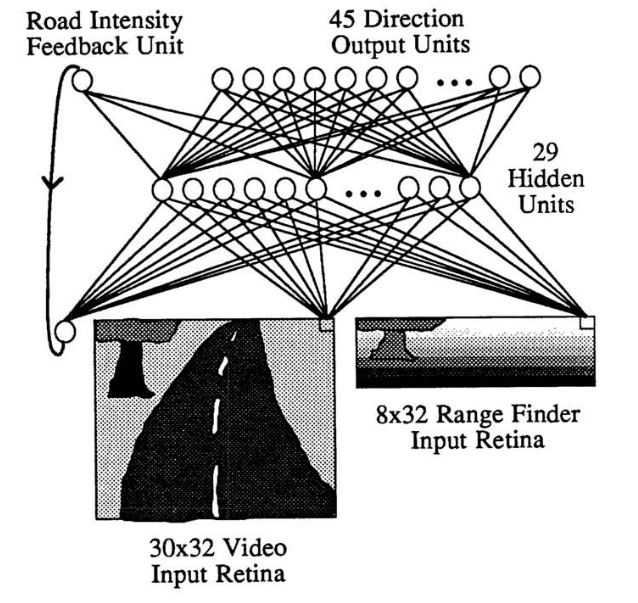
\includegraphics[height=8cm,page=1]{../img/alvinn_architecture.png}
    \caption{ALVINN modeļa uzbūve\cite{pomerleau1989alvinn}}
\end{figure}

Modeļa izvades slānis apzīmē vēlamo stūrēšanas virzienu 45 diskrētos soļos. Treniņa datu kopā faktisko virziena komandu atspoguļo neprecizēta veida ``zvana'' funkcija ar modu pie pareizā virziena. Ieviests viens papildus perceptrons, kas (teorētiski) novērtē ceļa gaišumu salīdzinot ar apkārtējo vidi, un tiek pievienots nākamās iterācijas ievades vektoram.

Jau šim (šķietami) samērā vienkāršajam uzdevumam konstatēts, ka ievākt treniņa datus fizikālā vidē --- braucot ar automašīnu pa ceļiem un ierakstot vadītāja veiktās korekcijas --- nav praktiski, jo nepieciešama ļoti liela treniņa datu kopa. Jāatzīst, ka ar modernākiem tehniskās redzes modeļiem droši vien šī nepieciešamība mazinātos. Tāpēc dati ģenerēti sintētiski --- tā kā gan video, gan attāluma datu izšķirtspēja ir gaužām neliela, pat ar 1989. gadā pieejamām datorgrafikas iespējām šādi gūtus attēlus ir grūti atšķirt no īstiem. Simulatorā iegūtie attēli un vadības komandas izmantoti klasifikatora apmācībā.

Iegūtais rezultāts --- modelis, kas maksimāli tuvināts simulatorā realizētajam kontroles algoritmam izmantotā šablona iespēju robežās. Tas bijis pietiekami labs, lai spētu vadīt ar kameru un attāluma sensoru aprīkotu automobili pa 400m garu slēgta ceļa posmu saulainos dienas apstākļos, ar ātrumu 0,5m/s. Tas tiek lietots kā arguments par neironu tīklu pavērtajām iespējām pašbraucošo auto attīstībā, taču netiek slēpts, ka sasniegtais ir tālu no praktiskas vadības sistēmas.

Kā galvenais uzvedības klonēšanas trūkums parasti tiek minēta nespēja atgūties no faktiskā stāvokļa sadalījumu nobīdes\cite{attia2018global} (\textit{distribution shift}). Ja reālais modelis $\pi_{\theta}(s)$ nevar pilnīgi precīzi atdarināt eksperta $\pi^*(s)$ darbības vai MDP pārejas funkcija ir stohastiska, tātad treniņa datu kopa neietver visas iespējamās trajektorijas ar atbilstošajām $\pi^*(s)$ vērtībām, $\pi_{\theta}$ inducētais stāvokļu sadalījums diverģē no $\pi^*$ inducētā. Lai iegūtu precīzāku un robustāku eksperta stratēģijas atdarinājumu, piedāvāti dažādi --- sarežģītāki --- apmācības paņēmieni.


\subsubsection{Statistiskas korekcijas}

Viens no virzieniem, kurā vesti centieni uzlabot trajektorju kopēšanas lietderību, ir strukturēt treniņa datu ieguvi un apmācības algoritmu veidā, kas maksimāli tuvina $\pi^*$ un $\pi_{\theta}$ inducētos stāvokļu sadalījumus. Bieži vien tas nozīmē, ka vienkārši ievākt datus un veikt apmācību uz tiem vairs nav iespējams --- nepieciešama aktīva instruktora iesaiste. Piedāvātie risinājumi ir dažādi, un metodes var kļūt visnotaļ sarežģītas\cite{attia2018global}, tāpēc, lai ilustrētu pieejas būtību kopumā, izvēlēts viens, vairāk teorētisks piemērs.

DAgger --- \textit{dataset aggregation} --- ir 2011. gadā publicētajā rakstā ``\textit{A Reduction of Imitation Learning and Structured Prediction
to No-Regret Online Learning}''\cite{ross2011no}, kā autori atkal ir no Kārnegija-Melona Universitātes ASV, piedāvāts algoritms. Tas piedāvā teorētiskas garantijas $\pi^*$ un $\pi_{\theta}$ inducēto sadalījumu konverģencei, kombinējot instruktāžu ar apmācāmā modeļa ģenerētām stratēģijām. Lai gan raksts nedarbojas tieši ar robotiku, izmantotais MDP kontroles formālisms ir vispārīgs.

Algoritma darbību var vienkāršoti aprakstīt sekojoši: pieņem, ka ir pieejami ne tikai eksperta ģenerēti trajektoriju dati, bet ir iespējams pašam ekspertam uzdot vaicājumus par katrā stāvoklī optimālu darbību --- kas, ja instruktāžu nodrošina cilvēks un laika soļu pārejas ir biežas, reti kad būs praktiski iespējams. Tādā gadījumā iteratīvi atkārto šādus soļus:

\begin{enumerate}
    \item ar kādu varbūtību $\alpha$ izvēlas, vai i-tā trajektorija tiks ģenerēta ar $\pi^*$ vai $\pi_{\theta}$;
    \item iegūtās laikrindas stāvokļa elementiem $s_t$ atrod atbilstošo $a^*_t=\pi^*(s_t)$ 
    \item kopējai datu kopai $D$ pievieno $D_i=\lbrace (s_1, a^*_1),... \rbrace$
    \item apmāca modeli $\pi_{\theta}$ uz papildinātās datu kopas
\end{enumerate}

Kā jau minēts, liela daļa raksta satura veltīta tieši algoritma teorētisko īpašību pierādīšanai, taču beigās arī veikti daži eksperimenti --- divi ar personāžu vadību dator-spēļu vidē, viens ar rokraksta zīmju atpazīšanu teksta virknēs. Lai gan visos gadījumos DAgger pārspēj uzvedības klonēšanas (vienkāršas $\pi^*$ aproksimēšanas no treniņa datu kopas) rezultātus, tā lietderību stipri ierobežo instruktora interaktivitātes prasības --- praksē reti kad ir iespējams kaut kas analoģisks datorspēļu aģentu treniņam izmantotajam simulatoram, kas ar dziļu pārlasi atrod labas stratēģijas jebkuram stāvoklim.

\subsubsection{Inversā stimulētā mācīšanās}

Cits veids, kā atdarināt instruktora dotas trajektorijas, ir pieņemt, kas tā stratēģija optimizē kādu slēptu atdeves funkciju $R^*(s)$ un mēģināt to atjaunot no pieejamās informācijas. Šādā veidā ar stimulētās mašīnmācīšanās metodēm var iegūt meklēto rezultā-tu. Kā jau parasti, iespējami dažādi veidi, kā formalizēt uzdevumu un tehniski to realizēt. 2004. izdotais ``\textit{Apprenticeship learning via inverse reinforcement learning}''\cite{abbeel2004apprenticeship} no Džordžijas Tehnoloģiju institūta, viens no citētākajiem rakstiem par šo tēmu (lai arī ne pirmais), piedāvā iteratīvu algoritmu nezināmas atdeves funkcijas atjaunošanai un izmantošanai. Galvenā atkāpe no tipiska MDP formālisma ir pieņēmums, ka nezināmā atdeves funkcija $R^*$ ir formā, 

\begin{equation}
    R^*(s) = w^* \cdot \phi(s)
\end{equation}

kur $w^*$ --- svaru vektors, bet $\phi: S \rightarrow [0,1]^k$ --- zināmu atribūtu izpausme noteiktos stāvokļos. $\phi$ nozīme ir tāda, ka ir iespējams noteikt, kādu sakarību lineāra kombinācija varētu būt īstā atdeves funkcija. Kā piemērs tiek piedāvāts autovadītāja uzdevums --- viens no atribūtiem varētu būt 1, ja mašīna atrodas uz ceļa, bet 0 citādi, u.t.t. $m$ treniņa kopas trajektorijām aprēķina vidējo faktoru vērtību summu, izteiktu kā

\begin{equation}
    \mu^* = \frac{1}{m}\sum_{i=1}^m\sum_{t=1}^T \gamma^t \phi(s^i_t)
\end{equation}

Tad tiek iteratīvi atkārtota procedūra, kur atrod kādu svaru vektoru $w^{i}$ un attiecīgi empīrisku atdeves funkciju $R^{i}(s) = {w^{i}}^T\phi(s)$, ko izmanto, lai apmācītu jaunu stratēģiju $\pi^i$. Tad šai stratēģijai atrod vidējo vērtību $\mu^i$ analoģiski (2.3), un visas iepriekšējās $\mu^{j \leq i}$ tiek izmantotas, lai atrastu nākamo svaru vektoru $w^{i+1}$. Process turpinās, līdz ir konverģējis līdz noteiktam kļūdas hiperparametram. Tādējādi beigās iegūta stratēģija, kas maksimizē līdzīgu atribūtu $\phi(s)$ kombināciju nezināmajai instruktora stratēģijai, un robusti seko demonstrācijām.

Rezultāti parāda, ka šī metode pārspēj dažādas vienkāršas, statistiskas $\pi^*$ aproksi-mācijas metodes (uzvedības klonēšanu). Kopā risināti divi dažādi uzdevumi. Viens ir ``\textit{gridworld}'' --- spēle, kurā aģents pārvietojas pa režģa formas vidi un dažos lauciņos ir pieejamas atdeves. Taču pārejas process ir stohastisks, tāpēc metodes, kas atdarina tikai telpiskos pārvietojumus un nemēģina atjaunot slēpto atdeves funkciju darbojas sliktāk. Otrs ir divdimensionāla spēle, kurā aģents vada automobili. Šeit tika pārbaudīts, vai var iemācīt aģentam atšķirīgus ``braukšanas stilus'' tikai ar demonstrācijām, kas arī izdevies.

\subsubsection{Uzdevumu simboliska dekompozīcija}

Vēl viena metode atdarināšanas spēju uzlabošanai ir telpisku kustības trajektoriju pārvēršana simbolisku, diskrētu darbību virknē. Pamatideja ir tāda, ka vieglāk iemācīties robusti izpidlīt primitīvas kustības un tad šādu primitīvo kustību secību kāda uzdevuma izpildē, nekā no neliela demonstrācija skaita iemācīties katru uzdevumu pilnībā no jauna. Šī arī nebūt nav jauna ideja --- izteikta jau 1980s un 1990os gados\cite{muench1994robot}. Jau 2002. gadā veikti pētījumi par algoritmiem, kas ļauj aproksimēt trajektorijas elementus ar autonomu, nelineāru diferenciālvienādojumu sistēmām\cite{ijspeert2002movement} un iemācīt pietiekami sarežģītas kustības --- piemēram, tenisa bumbas sišanu --- ar samērā nedaudziem piemēriem (ap 20). Ap to pašu laiku piedāvātas arī pieejas šādu primitīvu kustību kombinēšanai\cite{schaal2003computational}.

Pirms nesenā ļoti lielu neironu tīklu modeļu popularitātes uzplaukuma, šķiet, tieši simboliskās dekompozīcijas metodes bijušas starp perspektīvākajām. Robotikas literatūrā pirms 2010. gada\cite{billard2008handbook} gari un plaši rakstīts par šādiem paņēmieniem, taču pēdējos gados šī popularitāte varētu būt sarukusi. Jebkurā gadījumā, aktīva pētniecība nozarē vēl joprojām notiek, it sevišķi pielietojumiem, kur robots tiek mācīts ar kinestētiskām metodēm. Piemēram, ``\textit{A Framework of Hybrid Force/Motion Skills Learning for Robots}'' \cite{wang2020framework}, kas publicēts 2020. gadā, šāda pieeja tiek veiksmīgi izmantota uzdevumiem, kur svarīga ne tikai telpiskā trajektorija, bet arī uz apkārtējo vidi izdarīto spēku profils (piemēram, galda tīrīšanā).


\subsection{Novērojumu atdarināšana}

\subsection{Adaptīvu un atdarinošu metožu kombinācija}


\newpage
\section{Praktiska realizācija - rīki, piemēri}

\subsection{Simulācijas vides un saskarne}

\subsection{Vienkāršu modeļu realizācijas individuālai izpratnei}

\subsubsection{Stimulētā mašīnmācīšanās}

\subsubsection{Uzvedības kopēšana}

\subsubsection{DAgger}

\newpage
\section*{Secinājumi}
\addcontentsline{toc}{section}{Secinājumi}




\newpage
\printbibliography[title=Atsauces]
\addcontentsline{toc}{section}{Atsauces}

\end{document}